\documentclass[twocolumn,10pt,a4j]{jsarticle}
\usepackage{kougai}
\usepackage{dcolumn}


\title{シミュレータ教材開発に関する一提案}
\author{1532040 岡本 悠祐  指導教員 須田 宇宙 准教授}
\date{}
 
\begin{document}
\maketitle
\section{はじめに}
シミュレータ教材は不可視現象を可視化する教材であり,イメージが困難な事象の理解を促す手法として有用である.
e-Learningの普及に伴いシミュレータ教材の活用の場が増加し,様々な分野に対応したシミュレータ教材が求められ,処理速度だけでなく,効率的な開発手法が必要とされている.

本研究室では昨年,高負荷なシミュレータ教材にプログラマブルシェーダを利用し,GPUで動作された,CPUとの処理速度を比較する研究が行われた\cite{book}.
その結果,教材の処理速度は大幅に向上したが,ソースコードの変更箇所が多く,複雑なため,容易に実装できないという問題点が浮上した.

この問題点はWebWorkerによるマルチスレッド化と,サブスレッドから直接描画を行うOffscreenCanvasを利用することで緩和できると考られる.

そこで本研究では,OffscreenCanvasを利用したシミュレータ教材の開発を行い,ソフトウェアの生産性と処理速度の観点から有用性の検証を行うことを目的とする.

\section{比較に用いるシミュレータ教材}
\begin{figure}[b]
\vspace{-5mm}
 \begin{minipage}{0.49\hsize}
  \centering
  \vspace{-10mm}
   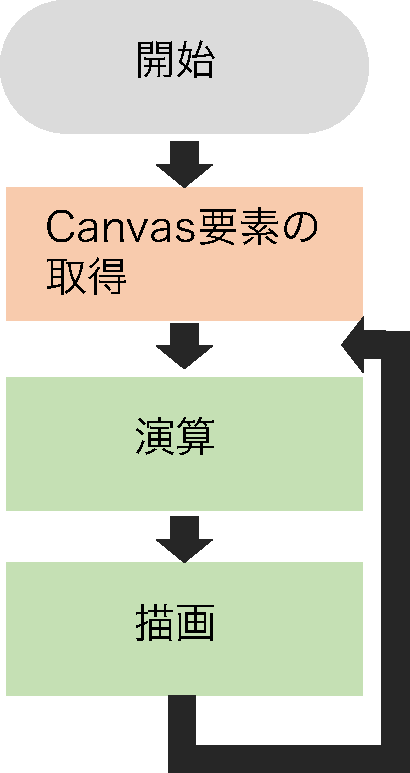
\includegraphics[width=23mm]{cpu_chart.pdf}
   \vspace{10pt}
  \caption{手法1のフローチャート}
  \label{fig:cpu}
 \end{minipage} 
 \begin{minipage}{0.5\hsize}
 \centering
  \vspace{5pt}	
  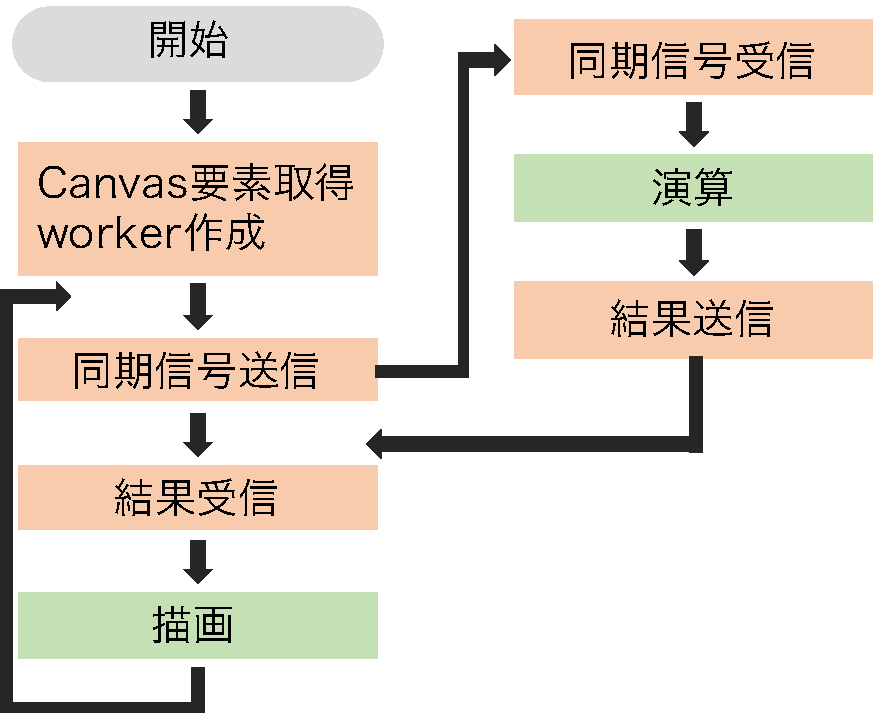
\includegraphics[width=40mm]{worker_chart2.pdf}
     \belowcaptionskip=25pt
  \abovecaptionskip=5pt
  \caption{手法3のフローチャート}
  \label{fig:worker}
 \end{minipage}
 
 \begin{minipage}{0.5\hsize}
 \centering
 \vspace{-25pt}	
  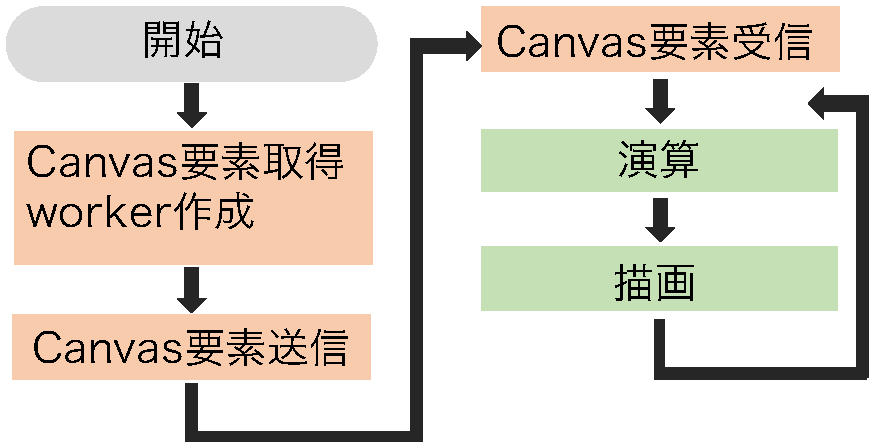
\includegraphics[width=45mm  ]{offsc_chart2.pdf}
  \abovecaptionskip=30pt
  \belowcaptionskip=-10pt
  \caption{手法4のフローチャート}
  \label{fig:offsc}
 \end{minipage}
 \begin{minipage}{0.49\hsize}
 \vspace{-14mm}
  \centering
   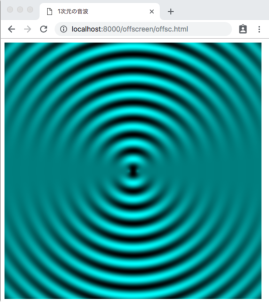
\includegraphics[width=35mm , angle=-90]{sim.pdf}
   \vspace{15pt}
  \caption{開発したシミュレータ}
  \label{fig:sim}
 \end{minipage}
\end{figure}
OffscreenCanvasの有用性の検証を行うにあたり,昨年度の卒業研究で使われた複数の音源から発せられる音場シミュレータを参照した.
昨年度に開発されたプログラムの内,JavaScriptのみで書かれたプログラムを手法1,GLSL(OpenGL Shading Language)で書かれたプログラムを手法2とする.

手法1のフローチャートを図\ref{fig:cpu}に示す.
1ピクセルごとに音源から発せられる音圧を求め,この処理を1フレームごとに繰り返し演算を行い,音圧を明暗で表現する.

手法1をマルチスレッド化したものを手法3とする.
手法3のフローチャートを図\ref{fig:worker}に示す.
演算をサブスレッドで実行するため,サブスレッドを多数作成することで高速化が期待できる.
しかし,サブスレッドでは描画を行えないため,メインスレッドに演算結果を送信する必要が生じる.

手法3にOffscreenCanvasを取り入れ,サブスレッドから直接描画する手法を手法4とする.
手法4のフローチャートを図\ref{fig:offsc}に示す.


手法4を用いて開発したシミュレータを図\ref{fig:sim}に示す.
Canvas要素を縦に2分割し,それぞれ別スレッドで計算・描画を行っている.

%%図\ref{fig:cpu}は手法1のフローチャートである.
%
%図\ref{fig:worker}は手法3のフローチャートである.mainでサブスレッドを定義することで,手法1をマルチスレッド化した.その際,mainからWorkerへデータの送信が必要となり,追加した.また,WebWorkerでは描画を行うことができないためWorkerで行った演算の結果をmainに送信し,mainで描画を行う必要があった.
%
%図\ref{fig:offsc}は手法4のフローチャートである.手法3を利用し,worker内での描画を可能とした.そのため,Workerでは演算の結果をmainに送信していたが,演算結果の送信を必要とせず,Worker内で演算と描画を完結させることができる.


\section{検証}
4つの手法の処理時間と,プログラムの追加・変更箇所の比較を行った.
処理時間はCPU:Intel Core i5 3.2GHz,GPU:NVIDIA GeForce GT 775Mを搭載したパソコンを利用し,10,000回演算を行う時間を計測した.
その結果を表\ref{tab:tab2}に示す.

手法3,手法4は複数のスレッドを用いて演算処理を行っているため処理速度が向上した.

%図\ref{fig:cpu}〜\ref{fig:offsc}より手法3,手法4のプログラムは,サブスレッドへデータの送信を行う処理を追加した.
%更に,手法3はサブスレッドから演算の結果をスレッドへ送信する処理を追加した.
%
%手法3は手法1の演算と描画が分離しているため,スレッドとサブスレッドの間で送受信が何度も行われた.
図\ref{fig:cpu}〜\ref{fig:offsc}より手法3はメインスレッドからサブスレッドへ演算データの送信とスレッドへ結果を送信する処理を追加した.

一方手法4はサブスレッドへCanvas要素の送信を行い,演算・描画処理を行った.
演算と描画が同じサブスレッド内で完結するため,繰り返しデータの送受信を行う必要がなく,処理1のソースコードの原型を崩さずに移植が行えた.

プログラムの変更箇所はHTMLでキャンバス要素を追加,描画範囲の指定を行うことで実装できた.

\begin{table} [htbp]
\vspace{6pt}
\centering
\caption{各種法の処理時間と時間比}
\vspace{4pt}
	\begin{tabular} {| c | c | c | } \hline
	手法 & 処理時間  (s)  & 時間比 \\ \hline
	1 & 206.6 & 1 \\ \hline 
	2 & 128.6 & 0.62 \\ \hline
	3 & 164.3 & 0.8 \\ \hline
	4 & 98.0 & 0.47 \\ \hline
	\end{tabular} 
	\label{tab:tab2}
\end{table}

\section{おわりに}
本研究ではシミュレータ開発におけるOffscreenCanvasの有用性を生産性と処理速度の観点から検証した.手法3,手法4共に処理速度が向上し,サブスレッドで演算だけ行うことより容易に実装が可能であることがわかった.今後はOffscreenCanvasを利用したシミュレータ教材の開発が増加することが予測される.
\begin{thebibliography}{99}

	\bibitem{book}中嶋 大貴:``GPU利用によるシミュレータ教材の演算速度'',平成29年度卒業論文,(2018)
\end{thebibliography}
\end{document}
